\section{Supporting comparisons and execution interpretation}
\label{sec:core_tables}
The following tables retain the exact core comparisons behind the main narrative. Seed standard deviations measure training variability; they are not respondent confidence intervals. The same-task API decomposition uses common respondent resamples and refers to a later Pro service, not a recovered training backend.
\begin{table}[pos=htbp]\centering\small
\centering\small
\caption{Probability-response fidelity on the held-out Teacher benchmark.}
\label{tab:response_main}
\setlength{\tabcolsep}{4pt}
\renewcommand{\arraystretch}{1.12}
\begin{tabular*}{\linewidth}{@{\extracolsep{\fill}}lrrr@{}}
\toprule
Model / objective & Macro-source KL $\downarrow$ & Response error $\downarrow$ & Interaction error $\downarrow$ \\
\midrule
Soft KL & $0.0915\pm0.0187$ & $0.0693\pm0.0032$ & $0.0457\pm0.0038$ \\
CE+KL & $0.1046\pm0.0170$ & $0.0753\pm0.0016$ & $0.0518\pm0.0038$ \\
Signed response & $0.0871\pm0.0138$ & $0.0665\pm0.0050$ & $0.0465\pm0.0036$ \\
Direction+magnitude & $0.0861\pm0.0145$ & $0.0659\pm0.0042$ & $0.0464\pm0.0039$ \\
\midrule
MNL-S & $0.0731$ & $0.0564$ & $0.0386$ \\
\bottomrule
\end{tabular*}
\par\smallskip\begin{minipage}{\linewidth}\footnotesize
Neural entries are means $\pm$ SD over three training seeds. The test set contains 437 states, 398 response pairs and 94 interaction contrasts from six held-out synthetic personas. All models, including the MNL-S regularization, are selected by validation macro-source KL. MNL-S uses the same inputs and training states as the neural Students.
\end{minipage}
\end{table}

\begin{table}[pos=htbp]\centering\small
\centering\small
\caption{Departure prediction under a common selection criterion (validation MAE).}
\label{tab:timing_main}
\setlength{\tabcolsep}{4pt}
\renewcommand{\arraystretch}{1.12}
\begin{tabular*}{\linewidth}{@{\extracolsep{\fill}}llrr@{}}
\toprule
Choice model & Departure predictor & Total parameters & MAE (min) $\downarrow$ \\
\midrule
Joint / soft KL & Shared neural encoders & 24,562 & $7.61\pm0.75$ \\
Joint / CE+KL & Shared neural encoders & 24,562 & $7.43\pm0.91$ \\
Joint / signed response & Shared neural encoders & 24,562 & $7.71\pm0.66$ \\
Joint / direction+magnitude & Shared neural encoders & 24,562 & $7.55\pm0.80$ \\
\midrule
MNL-S & Ridge regression & 555 & $12.35$ \\
MNL-S & Bounded linear & 555 & $11.19\pm1.24$ \\
MNL-S & Independent neural & 18,733 & $7.61\pm0.72$ \\
\bottomrule
\end{tabular*}
\par\smallskip\begin{minipage}{\linewidth}\footnotesize
Errors are measured against Teacher departure targets on the 437 test states. Neural and bounded-linear predictors report means $\pm$ SD over three training seeds, and the ridge fit is deterministic. MNL-S choice probabilities are identical across the three timing predictors. The joint models in this table are trained separately and selected by validation departure MAE, whereas those in Table~\ref{tab:response_main} are selected by validation KL.
\end{minipage}
\end{table}

\begin{table}[pos=htbp]\centering\small
\caption{Choice accuracy, PT share bias and mean absolute response bias against stated choices.}
\label{tab:human_main}
\setlength{\tabcolsep}{3pt}
\renewcommand{\arraystretch}{1.12}
\begin{tabular*}{\linewidth}{@{\extracolsep{\fill}}lrrrrrr@{}}
\toprule
& \multicolumn{3}{c}{Singapore ($n=332$)} & \multicolumn{3}{c}{Shanghai ($n=321$)} \\
\cmidrule(lr){2-4}\cmidrule(l){5-7}
Model & Acc. (\%) & PT bias (pp) & Mean $|B_c|$ & Acc. (\%) & PT bias (pp) & Mean $|B_c|$ \\
\midrule
SA-Student & $66.9$ & $-30.7$ & $4.0$ & $80.5$ & $-16.8$ & $5.8$ \\
MNL-S & $71.1$ & $-3.8$ & $11.1$ & $81.8$ & $-5.4$ & $4.1$ \\
Soft KL & $72.9\,\pm\,0.9$ & $-17.7\,\pm\,3.3$ & $8.2\,\pm\,3.3$ & $78.5\,\pm\,1.7$ & $-12.3\,\pm\,7.9$ & $7.6\,\pm\,0.9$ \\
CE+KL & $69.7\,\pm\,0.3$ & $-23.5\,\pm\,3.5$ & $6.9\,\pm\,1.7$ & $77.1\,\pm\,3.0$ & $-15.0\,\pm\,6.8$ & $9.1\,\pm\,1.9$ \\
Signed response & $73.1\,\pm\,1.2$ & $-16.0\,\pm\,3.5$ & $8.6\,\pm\,3.0$ & $79.8\,\pm\,1.1$ & $-10.7\,\pm\,6.2$ & $7.7\,\pm\,1.8$ \\
Direction+magnitude & $71.8\,\pm\,3.1$ & $-16.7\,\pm\,6.2$ & $8.8\,\pm\,2.0$ & $80.3\,\pm\,0.5$ & $-10.4\,\pm\,5.9$ & $7.5\,\pm\,1.0$ \\
\bottomrule
\end{tabular*}
\par\smallskip\begin{minipage}{\linewidth}\footnotesize
All 3,320 Singapore and 3,208 Shanghai explicit choices are scored, including eight and two choices of modes the model treats as unavailable. PT bias is the mean predicted PT probability minus the stated PT share. Mean $|B_c|$ is computed within each fitted seed by taking the absolute bias for each contrast and averaging over the five Singapore or eight Shanghai contrasts; these seed-level metrics are then averaged. Figure~\ref{fig:human_response} instead plots signed biases averaged over seeds, whose absolute values need not equal the table metric. Both are in percentage points. Neural entries are means $\pm$ SD over three training seeds. Always predicting PT gives accuracies of 66.57\% and 71.98\%. Further metrics are given in Supplementary Table~\ref{supp-tab:human_primary}.
\end{minipage}
\end{table}

\begin{table}[pos=htbp]
\centering\small
\caption{Decomposition of signed response differences among stated choices, the contemporary Teacher and SA-Student.}
\label{tab:teacher_decomposition_s9}
\setlength{\tabcolsep}{3pt}
\renewcommand{\arraystretch}{1.12}
\begin{tabular*}{\linewidth}{@{\extracolsep{\fill}}lrrr@{}}
\toprule
Contrast & Teacher $-$ human & SA-Student $-$ Teacher & SA-Student $-$ human \\
\midrule
\multicolumn{4}{l}{\textit{Singapore ($n=24$)}} \\
Poorer PT access & $+22.1\;[-9.9, 52.1]$ & $+1.9\;[-4.9, 9.1]$ & $+24.0\;[-7.2, 54.3]$ \\
Rain (active modes) & $+16.7\;[-2.4, 38.4]$ & $-5.0\;[-11.4, 1.1]$ & $+11.7\;[-8.0, 33.9]$ \\
PT fare & $-9.6\;[-33.4, 14.8]$ & $+7.8\;[4.1, 12.4]$ & $-1.8\;[-26.2, 22.6]$ \\
PT delay & $+1.9\;[-25.2, 28.9]$ & $-2.9\;[-12.3, 5.8]$ & $-0.9\;[-28.8, 29.7]$ \\
Road penalty & $+12.5\;[-12.0, 36.3]$ & $-1.0\;[-5.8, 4.2]$ & $+11.4\;[-14.8, 37.0]$ \\
\midrule
\multicolumn{4}{l}{\textit{Shanghai ($n=24$)}} \\
Rain & $-20.2\;[-41.6, -2.5]$ & $+3.0\;[-2.9, 8.0]$ & $-17.2\;[-41.5, 2.3]$ \\
PT delay & $+0.2\;[-10.2, 18.0]$ & $-26.7\;[-36.9, -15.4]$ & $-26.5\;[-39.3, -8.3]$ \\
Rain $\times$ delay & $+5.3\;[-13.9, 26.1]$ & $+9.7\;[3.3, 16.2]$ & $+15.0\;[-2.5, 34.7]$ \\
PT fare & $+0.0\;[-16.8, 16.7]$ & $+1.8\;[0.3, 3.2]$ & $+1.8\;[-14.6, 18.3]$ \\
Parking & $+7.0\;[-3.0, 24.6]$ & $-4.5\;[-11.0, -0.3]$ & $+2.6\;[-8.1, 17.7]$ \\
Road penalty & $+3.8\;[-10.3, 20.1]$ & $-1.5\;[-4.7, 0.7]$ & $+2.2\;[-11.6, 18.3]$ \\
Walk versus wait & $+16.3\;[0.2, 39.6]$ & $-11.9\;[-14.2, -9.1]$ & $+4.4\;[-13.0, 29.2]$ \\
Transfer versus wait & $+17.9\;[-7.4, 44.4]$ & $+2.9\;[0.4, 5.2]$ & $+20.8\;[-4.0, 46.8]$ \\
\bottomrule
\end{tabular*}
\par\smallskip\begin{minipage}{\linewidth}\footnotesize
Entries are percentage points with Bonferroni-adjusted respondent-bootstrap intervals, computed within each city over five Singapore or eight Shanghai contrasts. All terms use the same respondents, the same fitted SA-Student and Teacher means over three elicitations. Point estimates are rounded to one decimal place. The SA-Student $-$ Teacher term may include changes in the Teacher since training.
\end{minipage}
\end{table}

\begin{table}[pos=!ht]
\centering\small
\caption{Predicted and simulated PT responses in the fixed 1,000-person Helsinki population.}
\label{tab:execution_main}
\setlength{\tabcolsep}{3pt}
\renewcommand{\arraystretch}{1.12}
\begin{tabular*}{\linewidth}{@{\extracolsep{\fill}}llrrrr@{}}
\toprule
Model & Assignment & Predicted (pp) & Simulated (pp) & Gap (pp) & Assignment SD \\
\midrule
SA-Student & Deterministic & $-13.10$ & $-12.30$ & $0.80$ & -- \\
SA-Student & Stochastic & $-13.10$ & $-14.17$ & $-1.07$ & 1.55 \\
SA-Student & Constrained & $-13.10$ & $-14.17$ & $-1.07$ & 1.40 \\
Soft KL & Deterministic & $-6.97\pm4.92$ & $-8.03\pm5.13$ & $-1.06\pm1.24$ & -- \\
Soft KL & Stochastic & $-6.97\pm4.92$ & $-6.97\pm3.32$ & $0.01\pm2.18$ & 0.27 \\
Soft KL & Constrained & $-6.97\pm4.92$ & $-7.06\pm3.41$ & $-0.08\pm2.04$ & 0.28 \\
Direction+magnitude & Deterministic & $-6.77\pm4.96$ & $-8.63\pm4.76$ & $-1.87\pm1.33$ & -- \\
Direction+magnitude & Stochastic & $-6.77\pm4.96$ & $-7.12\pm3.97$ & $-0.35\pm1.30$ & 0.35 \\
Direction+magnitude & Constrained & $-6.77\pm4.96$ & $-7.22\pm4.06$ & $-0.45\pm1.24$ & 0.32 \\
MNL-S + neural time & Deterministic & $-6.84\pm0.00$ & $-6.90\pm0.00$ & $-0.06\pm0.00$ & -- \\
MNL-S + neural time & Stochastic & $-6.84\pm0.00$ & $-6.63\pm0.00$ & $0.21\pm0.00$ & 1.10 \\
MNL-S + neural time & Constrained & $-6.84\pm0.00$ & $-6.67\pm0.00$ & $0.17\pm0.00$ & 1.21 \\
\bottomrule
\end{tabular*}
\par\smallskip{\footnotesize Responses are changes in PT use from baseline to perceived delay over the same 1,000 people, with the physical timetable unchanged. Gap is the simulated minus the predicted response. Constrained denotes feasibility-constrained stochastic assignment. Values average assignment repetitions within each fitted model and then across models, and $\pm$ gives the SD across three training seeds. SA-Student is a single fitted model. Assignment SD is the mean within-model SD across assignment repetitions. Intermediate stages and absolute-gap summaries are given in Supplementary Tables~\ref{supp-tab:execution_layers}--\ref{supp-tab:execution_gap_aggregation}.}
\end{table}


\FloatBarrier
\subsection{Assignment, routing and completion}
\label{sec:execution_support}
The original perceived-delay experiment contains 140 model--condition--assignment configurations, all with the full population retained. Its sampling policies use three paired assignment seeds; this differs from the five-seed four-arm extension. No run encountered zero retained feasible mass. If that mass is zero, the implementation stops rather than silently discarding the traveler. Behavioral predictions are computed once, followed by a departure adjustment, feasibility checks, assignment and routing at the adjusted time.

For SA-Student, the original feasibility-constrained result shifts the PT response by approximately $+0.27$ percentage points during probability adjustment and by $-1.34$ points between adjusted probabilities and boarding. The total gap is about $-1.07$ points. These values describe three assignment seeds and should not be interchanged with the five-seed extension. The new reanalysis averages paired seeds within person before estimating intervals for every stage increment; its full aggregate ledger is supplied with the article data. Signed averages can hide opposing model-level gaps, which is why the supplement also reports absolute gaps after averaging assignment repetitions within each fitted model.

The physical disruption groups scheduled trips by line and ordered stops, retains alternating departures chronologically, and keeps singleton groups. It retains 6,924 of 13,655 trips across 344 groups. The baseline level-of-service reconstruction matches all 1,000 inputs. Every one of the 40 extension configurations passes checks on population size, assignment transformation, common random numbers, supply paths and retained trip identifiers. Each completes all outbound journeys. Completion-conditioned and completion-or-horizon means therefore coincide in these runs, although neither is a calibrated real-world time estimate.
\subsection{Feasibility correction and response geometry}
\label{sec:feasibility_geometry}
For a normalized distribution $\mathbf p$ and feasible set $F$ with mass $Z>0$, conditional renormalization adds mass $1-Z$ within $F$ and removes mass $1-Z$ outside it. Hence $\|\mathbf q-\mathbf p\|_1=2(1-Z)$. Every distribution supported on $F$ must remove all outside mass, and its inside changes have a sum of $1-Z$; the triangle inequality therefore gives the same lower bound. Conditional renormalization attains it, though the $L_1$ minimizer need not be unique.

An endpoint-optimal correction need not preserve a paired response. For a fixed feasible set $F=\{1,2\}$, let baseline probabilities be $(0.4,0.3,0.3)$ and perturbed probabilities $(0.4,0.2,0.4)$. Their corrections are $(4/7,3/7,0)$ and $(2/3,1/3,0)$. The probability of mode 1 is unchanged before correction but increases by $2/21$ afterward. This constructed example proves the distinction without making a claim about its empirical prevalence. The main-text decomposition reports the specified correction separately from subsequent execution; it does not attribute every correction-induced response difference to an unavoidable lower bound.
\FloatBarrier
\subsection{Active-mode speed sensitivity in Shanghai}
\label{sec:speed_sensitivity}
The Shanghai experiment holds the 321 people, their assigned modes, departure times and plans fixed, and compares active-mode speeds derived from the network links with caps of 1.34 m/s for walking and 4.17 m/s for cycling. The timetable is the same in the baseline and perceived-delay conditions. PT users number 224 at baseline and 134 under delay, and every person completes both journeys.

With network-derived speeds, mean outbound times are 19.68 minutes at baseline and 15.23 minutes under perceived delay. With speed caps, the corresponding means are 33.59 and 47.63 minutes. The paired difference is therefore $-4.44$ minutes ($[-5.06,-3.84]$) under link speeds and $+14.04$ minutes ($[11.18,17.05]$) under speed caps (Figure~\ref{fig:speed_sensitivity}). Delay moves 90 travelers away from PT, and whether this shortens or lengthens the average journey depends on the speeds assumed for walking and cycling. The times are model outputs and have not been compared with observed trip durations.
\begin{figure}[pos=htbp]
\centering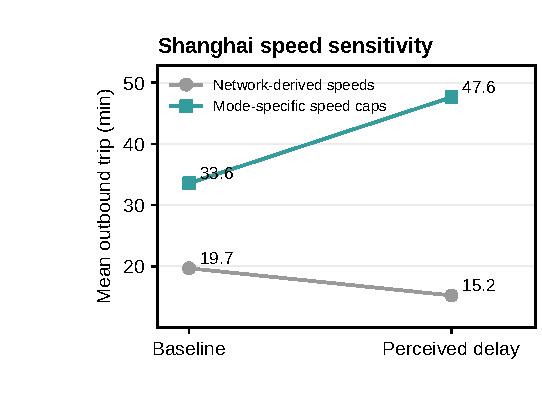
\includegraphics[width=.57\textwidth]{figures/narrative/figureS_speed_sensitivity.pdf}
\caption{Sensitivity of Shanghai journey times to the speeds of walking and cycling in the simulation. People, assigned modes, departure times and physical timetables are identical across speed settings. Values are mean durations of completed outbound trips.}
\label{fig:speed_sensitivity}
\end{figure}
